% !TeX root = ../Thesis.tex

\chapter{Theorie}\label{ch:Theory}
\section{Überblick}
Im nachfolgenden Kapitel wird der theoretische Hintergrund der vorliegenden Thesis behandelt. 
Hierzu werden sowohl für die Arbeit relevante Methoden als auch die Literatur verwandter Projekte und Studien zum aktuellen Stand der Technik beleuchtet. 
Da die Arbeit im Kern die panoptische Segmentierung von Zelldaten behandelt, werden hier Methoden zur Instanzsegmentierung und Klassifikation vorgestellt.
Die Methoden zur Instanzsegmentierung sind auf \ac{ki}-Methoden konzentriert; von klassischen Ansätzen wird abgesehen.
Für die Klassifikation wird von grundlegenden Erklärungen der Deep-Learning-Methoden abgesehen.
Stattdessen werden einzelne moderne Ansätze sowie relevante Methoden der Visualisierung oder Optimierung von Klassifikatoren angeführt.
Um die Methoden in einem vergleichbaren und reproduzierbaren Aufbau zu demonstrieren, werden zudem Benchmark-Methoden beleuchtet.
Dem theoretischen Hintergrund wird der Neuheitswert der Arbeit gegenübergestellt, um den Beitrag der vorliegenden Arbeit zur Forschung zu verdeutlichen.

\section{Methoden}
\subsection{Benchmark}
Um die Leistungsfähigkeit der im Rahmen der vorliegenden Thesis eingeführten Methoden zu prüfen, sind umfangreiche Datensätze erforderlich. 
Für jede isolierbare Aufgabe muss ein Datensatz gewählt werden, der Annotationen entsprechend dieser Aufgabe enthält.
Die Herausforderung bei der Auswahl eines Datensatzes besteht darin, dass die darin enthaltenen Daten (Quelldaten) den Daten \textit{ähnlich} sein müssen, für die die Anwendung entworfen wird (Zieldaten).
So wird sichergestellt, dass sich die auf den Quelldaten gemessene Qualität der Anwendung sinnvoll auf die Zieldaten übertragen lässt \cite{ganin2015domain_big}.
Der Begriff \textit{Ähnlichkeit} ist mehrdeutig, und das Definieren von Merkmalen in Daten, die \textit{Ähnlichkeit} messen, ist anspruchsvoll.
Metriken, die als Maß für \textit{Ähnlichkeit} herangezogen werden, müssen maßgeschneidert zur Anwendung passen und sind bereits breit erforscht \cite{zhu2020domain_similarity, koohi2018similarity, cai2009similarity}.
Daten können mithilfe passender Metriken \textit{Ähnlichkeits-}Gruppen, sogenannten \textit{Domänen}, zugeordnet werden \cite{yuan2005domainsimilarity}.
Beispiele für Domänenunterschiede in biomedizinischen Bildaufnahmen sind verschiedene Farbmarker, Aufnahmegeräte oder Zoomstufen. 
In Abb. \ref{fig:domains} sind Zellkerne verschiedener Domänen abgebildet. 
\begin{figure}[H]
    \centering
    \includegraphics[width=0.98\linewidth]{Figures/Cell_domains.pdf}
    \caption{Vier Aufnahmen von Zellen. Die Bilddomänen lassen sich durch die verschiedenen Marker und Aufnahmetechniken klar unterscheiden.
    a) 3D-Bildstapel aus den Daten der vorliegenden Arbeit mit verschiedenen Fluoreszenzmarkern, aufgenommen mit einem Leica TCS SP8 Konfokalmikroskop.
    b) 3D-SIM-Superauflösungsmikroskopie mit DAPI-Färbung \cite{Schermelleh2008}.
    c) Konfokale Fluoreszenzmikroskopie mit antikörperbasierten Farbstoffen \cite{Peng2015}.
    d) Klassische Hellfeldmikroskopie \cite{Ali2012}.}
    \label{fig:domains}
\end{figure}
\noindent
Intuitiv gehören die sichtbaren Objekte zur Klasse \textit{Zellkern}, aber der Stil unterscheidet sich stark. 
Sie unterscheiden sich also in ihrer jeweiligen Domäne.
In der Bildverarbeitung ist es essenziell, die Domäne der Quelldaten im Hinblick auf die Aufgabe der Applikation zu berücksichtigen \cite{wang2018domain, peng2017domain}. 
Hierzu kann ein Datensatz mit passender Domäne gewählt werden oder eine Domänenanpassung durchgeführt werden \cite{han2022binsimilarity_domain, pinheiro2018domain, ganin2016domain}. \\[0.5\baselineskip]
Ghosh et al. definieren Domänenanpassung: \glqq Gegeben Quell- und Ziel-Domänen $D_s$ und $D_t$ sowie die Aufgaben $\tau_s$ und $\tau_t$, zielen Domänenadaptations-basierte Verfahren darauf ab, ein Modell mit Parametern $\theta$ zu erlernen, das für die Zielaufgabe geeignet ist, wenn $D_s \neq D_t$ und $\tau_s = \tau_t$.\grqq \cite{Ghosh2020}.
\subsection{Segmentierung}\label{sec:Segmentierung}
Segmentierung ist die Aufgabe, Pixel mit semantischen Annotationen zu klassifizieren (semantische Segmentierung \cite{Hariharan2014}), einzelne Objekte voneinander abzugrenzen (Instanzsegmentierung \cite{Winn2006}) oder beides zu kombinieren (panoptische Segmentierung \cite{kirillov2019PQ}) \cite{Minaee2021}.
In Abb. \ref{fig:Segmentation} sind beispielhaft Annotationen der verschiedenen Segmentierungsarten zu sehen \cite{kirillov2019PQ}. 
Links zu sehen ist ein exemplarisches Originalbild. 
Daneben sind von links nach rechts Segmentierungsmasken für semantische, Instanz- und panoptische Segmentierung zu sehen. 
In der semantischen sowie in der panoptischen Maske sind die Farben der Objekte mit einer interpretierbaren Objektklasse verknüpft.\\ [0.5\baselineskip]
\begin{figure}[h!]
    \centering
    \includegraphics[width=\textwidth]{Figures/Segmentation_Types.pdf}
    \caption{Die verschiedenen Arten der Segmentierung. Links ist das Originalbild zu sehen, rechts sind die zugeordneten pixelweise Annotationen farblich eingezeichnet. 
    Gleiche Farben bedeuten gleiche Annotationen. 
    In der semantischen Maske sind gleiche Annotationen mehrerer Objekte derselben semantischen Klasse zu finden. 
    In der Instanz-Maske ist jedem Objekt eine individuelle Annotation zugeordnet, unabhängig von dessen Klasse. 
    In der panoptischen Maske sind auch einzelne Objekte getrennt, den Annotationen verschiedener Klassen werden allerdings noch semantische Klassen zugeordnet \cite{kirillov2019PQ}.}
    \label{fig:Segmentation}
\end{figure}
\noindent
Für die verschiedenen Segmentierungsarten werden Architekturen an die jeweilige Aufgabe angepasst \cite{Arnab2017, Chen2018}. 
Modelle sind dabei in der Regel nach dem Vorbild des \textit{U-Net} \cite{Ronneberger2015} aus einem Merkmalsextraktor (Encoder) und einem Vorhersagenetz (Decoder) aufgebaut \cite{Girshick2014}.
Der Encoder nutzt zur Merkmalsextraktion beispielsweise Bildfaltungen mit Kernen, deren optimale Gewichte anhand annotierter Daten gelernt werden \cite{Long2015}.
Dabei verringert der Encoder iterativ die Größe der Eingabe jeder Schicht des Netzes in X-, Y- und im dreidimensionalen Fall in Z-Richtung, erhöht dabei aber die Informationstiefe pro verbleibendem Pixel, bis ein hochdimensionaler Merkmalsvektor übrig bleibt. 
Der Decoder hebt, meist durch transponierte Bildfaltungen \cite{Zeiler2010, Zeiler2014}, die räumliche Auflösung schrittweise wieder an, indem er die Bilddimensionen vergrößert und die Merkmalskanäle gleichzeitig reduziert \cite{Noh2015}. 
Über sogenannte Skip connections \cite{Ronneberger2015} werden dabei Merkmale aus den entsprechenden Encoder-Schichten mit den Decoder-Stufen verknüpft, sodass sowohl globale Kontextinformationen als auch feine Strukturen für die Segmentierung erhalten bleiben \cite{Mostajabi2015, Gu2018}.\\ [0.5\baselineskip]
Zur Nachbearbeitung von Segmentierungsmasken kann das Watershed-Verfahren eingesetzt werden \cite{Belaid2009}.
Dabei wird zunächst aus der Segmentierungsmaske ein Gradientenbild erzeugt und anschließend eine Überflutungssimulation durchgeführt, bei der regionale Minima als Startpunkte dienen. 
Der Algorithmus eignet sich insbesondere zur Trennung überlagerter Instanzen.
\\ [0.5\baselineskip]
Biologische und medizinische Bilddaten sind oft dreidimensionale Volumina. 
Dreidimensionale Daten erhöhen sowohl den Rechenaufwand für die Segmentierung als auch die Komplexität von Segmentierungsmodellen und stellen damit eine besondere Herausforderung dar \cite{Taha2015, Zhang2022, Avesta2023a}.
Methoden für zweidimensionale Segmentierung lassen sich anpassen, um direkt mit dreidimensionalen Daten zu operieren \cite{Yang2021}.
Auch explizite \linebreak 3D-Segmentierungsmethoden werden erforscht \cite{Arnab2021, Wang2025}.
Da die Auflösung in Z-Richtung oft geringer ist als die räumliche Auflösung, werden häufig 2.5D-Methoden verwendet, die die Beziehungen zwischen Volumenschichten gesondert modellieren \cite{Hung2024}.
Auch 2D-Methoden werden für 3D-Segmentierung eingesetzt, indem einzelne 2D-Schichten des Volumens segmentiert und anschließend durch Nachverarbeitung zusammengefügt werden \cite{Karimi2024}.
Die besten Ergebnisse liefern in der Regel 3D-Methoden \cite{Avesta2023}.

\subsection{Klassifikation}\label{sec:Klassifikation}

Klassifikation beschreibt das Zuordnen einer Kategorie oder Klasse, zu der eine gegebene Stichprobe gehört \cite{Fukunaga1993}.
Hierzu werden die Merkmale des Objekts, das in der Stichprobe präsentiert wird, durch Beobachtung oder Messung erfasst \cite{Kulkarni1998}.
Nach wiederholter Extraktion der Merkmale von Objekten verschiedener Klassen werden Muster in den Merkmalen gesucht, um Regeln für die Zuweisung von Objekten zu Klassen auf Basis dieser Muster festzulegen \cite{Jain1999, ShalevShwartz2014}.
Sowohl die Algorithmen zur Merkmalsextraktion als auch zum Ableiten der Muster und Regeln können mit unterschiedlich hohem Rechenaufwand, Abstraktionsgrad und Maß an Generalisierbarkeit implementiert werden \cite{Loog2018}. 
Zur Merkmalsextraktion werden klassisch beschreibende Eigenschaften des Objekts berechnet und miteinander kombiniert \cite{Guyon2006}.
Als Eigenschaften eignen sich beispielsweise die Verteilung der Farbkanäle, eine Charakterisierung der Textur oder die Fläche des Objekts \cite{Kunaver2005, Mutlag2020}.
Eine weitere verbreitete Eigenschaft ist eine Kombination von Parametern der Fourier-Entwicklung einer Kontur, die aus der diskreten komplexen Zahlenfolge
\begin{equation}
  c[n] = x[n] + i \cdot y[n], \quad n = 0, \ldots, N-1\text{,}
\end{equation}
mithilfe der diskreten Fourier-Transformation 
\begin{equation}
  F[k] = \sum_{n=0}^{N-1} c[n] \cdot e^{-2 \pi i \frac{kn}{N}}, \quad k = 0, \ldots, N-1\text{,}
\end{equation} 
gebildet werden \cite{Zahn1972, Kuhl1982}.
Hierbei sind $x[n]$ und $y[n]$ die Koordinaten des $n$-ten von N equidistanten Sützpunkten entlang der Kontur des Objekts, $c[n]$ ihre komplexe Darstellung und $F[k]$ die Fourier-Transformation der komplexen Darstellungen.
Die Ergebnisse der Fourier-Transformationen mehrerer Stützpunkte werden anschließend als Eigenschaften verwendet.
Merkmalsvektoren werden häufig abstrahiert und in ihrer Dimensionalität reduziert, beispielsweise durch eine Principal Component Analysis \cite{Pearson1901, Hotelling1933}.
Sind keine Annotationen verfügbar, werden diese Metriken zum Clustering verwendet \cite{Jain1999, Xu2005}. 
Wenn nur wenige Annotationen vorhanden sind, können semi-supervised-Verfahren angewandt werden, die insbesondere die Ähnlichkeit zwischen Stichproben ohne Annotationen herausarbeiten \cite{Boser1992, Yarowsky1995}.
Eine prominente Methode des semi-supervised-Lernens ist das Label-Spreading, das mithilfe einer Kernfunktion \cite{Schoelkopf1997, Smola1998} die Dimensionen von Merkmalsvektoren ändert und in einen alternativen Merkmalsraum transformiert \cite{Zhou2003}.
Verschiedene Kernfunktionen wie die Radiale Basis Funktion \cite{Lowe1988}
\begin{equation}
    \phi(x, y) = \exp\!\left(-\gamma \|x - y\|^2\right), \quad \gamma > 0
\end{equation}
werden für das Label-Spreading eingesetzt \cite{Delalleau2005}.
Hierbei sind $x, y \in \mathbb{R}^d$ die Koordinaten der Stichprobe im Merkmalsraum, $\gamma$ ein Parameter, der die Breite der Radialbasisfunktion steuert, und $\phi(x,y)$ der Wert der Radialen-Basis-Funktion.
Die meist genutzten Methoden der Klassifikation sind logikbasierte Ansätze wie Entscheidungsbäume, Perzeptron-basierte Ansätze wie neuronale Netze, statistische Ansätze wie Bayes'sche Netzwerke oder Nächster-Nachbar-Verfahren und Support-Vector-Maschinen \cite{Kotsiantis2007}.
Diese Methoden basieren direkt auf Ähnlichkeiten zwischen den Merkmalen unbekannter Stichproben und Stichproben mit bekannter Klasse \cite{Hughes1968}.
Moderne Anwendungen nutzen zur Merkmalsextraktion verschiedene Deep-Learning-basierte Methoden \cite{Khan2023}.
Vor allem \linebreak \acp{cnn} \cite{Krizhevsky2012} und \acp{vit} \cite{Bain2021} können aus Bildern aussagekräftige, abstrakte Merkmale extrahieren \cite{Plested2022}.
Ein Netz, das zur Merkmalsextraktion eingesetzt wird, wird als \textbf{Encoder} bezeichnet. \\ [0.5\baselineskip]
Als \textbf{Klassifikations-Kopf} wird der zusammenfassende Teil des Klassifikators bezeichnet; er gibt einen Zuversichtlichkeitswert für jede Klasse aus.
Der State-of-the-Art für den Klassifikations-Kopf ist ein neuronales Netz, das auf Basis der abstrakten Merkmale des Encoders eine Zuversichtlichkeit für jede Klasse ausgibt \cite{Ghods2019}.
Hierzu lernt in der Regel ein Multi-Layer-Perzeptron auf Basis von Trainingsdaten mit zugehöriger Annotation den Zusammenhang zwischen den Merkmalen und der assoziierten Klasse \cite{Schmidhuber2015}.\\ [0.5\baselineskip]
Für das Training von Klassifikatoren sind eine Loss-Funktion und häufig Vorverarbeitungsmethoden erforderlich.
Der Cross-Entropy Loss \cite{Sukhbaatar2014} \newline
\begin{equation}
    \mathcal{L}(\theta) = \frac{1}{N} \sum_{n=1}^{N} 
    - \log p(\tilde{y} = \tilde{y}_n \mid x_n, \theta)
\end{equation}
ist die etablierte Loss-Funktion für das Training von Klassifikatoren \cite{GordonRodriguez2020, Mao2023}.
Hierbei ist der Loss $L$ von der Annotation $\tilde{y}$ und der Vorhersage $\tilde{y}_n$ abhängig, die von den Eingangsdaten $x_n$ und den Modellparametern $\theta$ bestimmt werden.  
Ein Problem der Cross-Entropy-Loss-Minimierung ist ihre Anfälligkeit gegenüber Rauschen in den Annotationen.
Viele verschiedene Ansätze in der Forschung gehen dieses Problem an \cite{Goldberger2017, Han2018, Hendrycks2018}.
Eine häufig genutzte Methode ist die Minimierung des Generalized Cross Entropy Loss \cite{Zhang2018}
\begin{equation} 
    \argmin_{\theta,\, w \in [0,1]^n} 
    \sum_{i=1}^{n} w_i \mathcal{L}_q(f(x_i; \theta), y_i) 
    - \mathcal{L}_q(k) \sum_{i=1}^{n} w_i,
\end{equation}
wobei $\mathcal{L}_q$ die generalisierte Form des Cross-Entropy-Losses ist, die durch den Parameter $q$ reguliert wird. 
Dieser kontrolliert den Einfluss fehlerhafter oder unsicherer Trainingsbeispiele.
Die Gewichte $w_i \in [0,1]$ dienen der Gewichtung einzelner, besonders unsicherer Trainingsinstanzen.
Das Modell $f(x_i; \theta)$ gibt die Vorhersage für die Eingabe $x_i$ basierend auf den Modellparametern $\theta$ aus, während $y_i$ die entsprechende Zielannotation ist.\\ [0.5\baselineskip]
Bilineare Interpolation ist ein Verfahren zur Bildvorverarbeitung, das die Bilddimension erhöht, indem Werte für neue Pixel zwischen bestehenden Pixeln geschätzt werden \cite{Smith1981}.
Zur Schätzung des neuen Wertes wird dabei ein gewichtetes Mittel aus den vier benachbarten Pixeln genommen:
\begin{equation}
\hat{f}(x,y) = (1-p)(1-q)f_{i,j} + p(1-q)f_{i+1,j} + (1-p)q f_{i,j+1} + pq f_{i+1,j+1},
\end{equation}
wobei $\hat{f}(x,y)$ der neue Wert, $p, q \in [0, 1]$ die relativen Abstände zu den Nachbarpixeln, $i, j$ die Indizes der Nachbarpixel und $f$ die Intensitäten der Nachbarpixel sind. \\ [0.5\baselineskip]
Normierungsmethoden werden während des Trainings eingesetzt, um die Daten zu regulieren und Signale weder unverhältnismäßig groß noch verschwindend klein werden zu lassen.
Batch normalization normalisiert die Eingänge einer Schicht über ein mini batch, indem für jedes abstrakte Merkmal der Schicht, das bei der Dimensionsreduktion des Bildes entsteht, eine Transformation durchgeführt wird \cite{Ioffe2015}.
Für die Transformation wird der Mittelwert des mini batches vom Wert abgezogen und durch die Standardabweichung geteilt.
Layer normalization verfolgt einen ähnlichen Ansatz, berechnet den Mittelwert und die Varianz aber pro Schicht von allen Neuronen \cite{Ba2016}.
Beide stabilisieren das Training tiefer neuronaler Netze und lassen die Normalisierung als Bestandteil der Modellarchitektur lernen, statt sie nur als Vorverarbeitungsschritt durchzuführen \cite{Santurkar2018, Xu2019}.\\ [0.5\baselineskip]
Als Vergleichsmetrik der Klassifikation wird für gewöhnlich die Genauigkeit des getesteten Netzes auf den annotierten Daten verwendet:
\begin{equation}
  \text{Genauigkeit} = \frac{1}{N} \sum_{i=1}^{N} \mathbf{1}\{\hat{y}_i = y_i\},
\end{equation}
wobei $N$ die Anzahl der Vorhersagen, $\hat{y}_i$ die Vorhersage des Klassifikators und $y_i$ die Annotation sind. \\ [0.5\baselineskip]
Um das Verhalten von Klassifikatoren zu visualisieren, gibt es verschiedene Methoden.
Eine dieser Methoden ist Grad-CAM \cite{Selvaraju2017}.
Grad-CAM steht für Gradient-weighted Class Activation Mapping und ist eine Methode, um räumlich aufgelöste Relevanzkarten aus tiefen neuronalen Netzen zu erzeugen. 
Dabei werden die Gradienten einer bestimmten Klasse bezüglich der Aktivierungen einer Schicht des Modells verwendet, um Regionen des Eingabebildes zu finden, die besonders stark zur Vorhersage beitragen. 
Die resultierende \glqq Wichtigkeits\grqq-Karte wird auf die Eingabe zurückprojiziert und wird typischerweise als farbige Heatmap dargestellt.
Abb. \ref{fig:gradCam_example} zeigt zwei Beispiele einer solchen Heatmap \cite{Selvaraju2017}.
\begin{figure}[H]
    \centering
    \includegraphics[width=0.75\linewidth]{Figures/gradCAM_example.pdf}
    \caption{Grad-CAM Beispiel.
    Links ist das Originalbild zu sehen.
    Daneben sind zwei Heatmaps platziert, die mit Grad-CAM die Wichtigkeit räumlicher Regionen des Bilds für die Klassen \glqq Katze\grqq und \glqq Hund\grqq visualisieren.}
    \label{fig:gradCam_example}
\end{figure}
\noindent
Mithilfe der extrahierten Gradientenkarten lassen sich neben der Wichtigkeit bestimmter räumlicher Regionen der Eingangsdaten auch die relative Wichtigkeit der Eingangskanäle bestimmen.
Durch die Integration des Gradientenfelds werden stabilere und interpretierbarere Aussagen möglich. 
Die Integration gleicht lokale Schwankungen der Gradienten aus.
Mithilfe der Kosinusähnlichkeit, die den Winkel zwischen zwei Vektoren im Merkmalsraum beschreibt und damit die Übereinstimmung ihrer Richtungen quantifiziert, werden die integrierte und die nicht integrierte Karte auf Konsistenz geprüft. 
Eine hohe Kosinusähnlichkeit weist darauf hin, dass beide Karten auf ähnliche Eingabemuster reagieren und das Modell intern konsistente Repräsentationen der relevanten Merkmale lernt.\\ [0.5\baselineskip]
Eine weitere Möglichkeit, die Effizienz eines Klassifikators zu visualisieren, ist ein Scatterplot, der den Merkmalsraum, in den der Klassifikator die Eingangsdaten abbildet, niederdimensional darstellt.
Im Scatterplot werden Stichproben aus verschiedenen Klassen eingetragen.
Die Clusterbildung im Scatterplot visualisiert, wie gut die Klassen im Merkmalsraum getrennt sind, und liefert eine Schätzung der Güte des Klassifikators auf den vorliegenden Daten.
Um den Merkmalsraum in eine visualisierbar niedrige Dimension zu projizieren, wird häufig die \ac{tsne} eingesetzt \cite{Maaten2008, Cai2022}.
Die \ac{tsne} ist eine nichtlineare Methode zur Dimensionsreduktion, speziell zur Visualisierung hochdimensionaler Daten in zwei oder drei Dimensionen.
Die Methode modelliert die Abstände zwischen den Datenrepräsentationen im hochdimensionalen Raum als Wahrscheinlichkeitsverteilungen und definiert eine Transformation in eine niederdimensionale Repräsentation mit den entsprechenden Wahrscheinlichkeitsverteilungen.
Mit einem Optimierungsalgorithmus minimiert die \ac{tsne} die Kullback-Leibler-Divergenz der beiden Wahrscheinlichkeitsverteilungen, um die Entfernungen der Datenpunkte in beiden Räumen möglichst ähnlich zu machen.
Abb. \ref{fig:scatter_tsne_example} zeigt exemplarisch zwei solcher Scatterplots für den MNIST-Datensatz \cite{Lecun1998}.
Die Scatterplots visualisieren den Merkmalsraum des gleichen Klassifikators nach einer Epoche des Trainings (links) und nach 25 Epochen des Trainings (rechts).
Links sind die Klassen-Cluster schlechter getrennt als rechts. 
\begin{figure}[H]
    \centering
    \begin{subfigure}[b]{0.49\textwidth}
        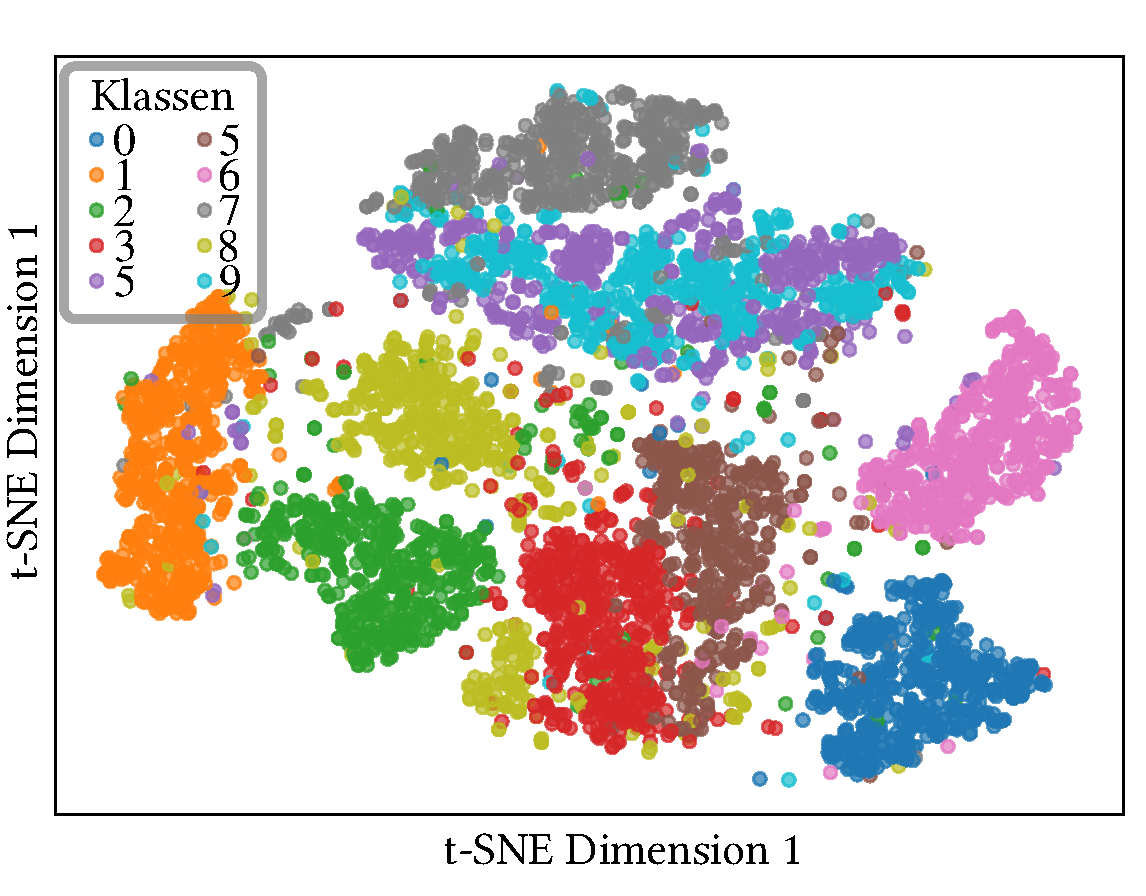
\includegraphics[width=\textwidth]{Figures/scatter_bad.pdf}
    \end{subfigure} 
    %\hspace{0.5cm}
    \begin{subfigure}[b]{0.49\textwidth}
        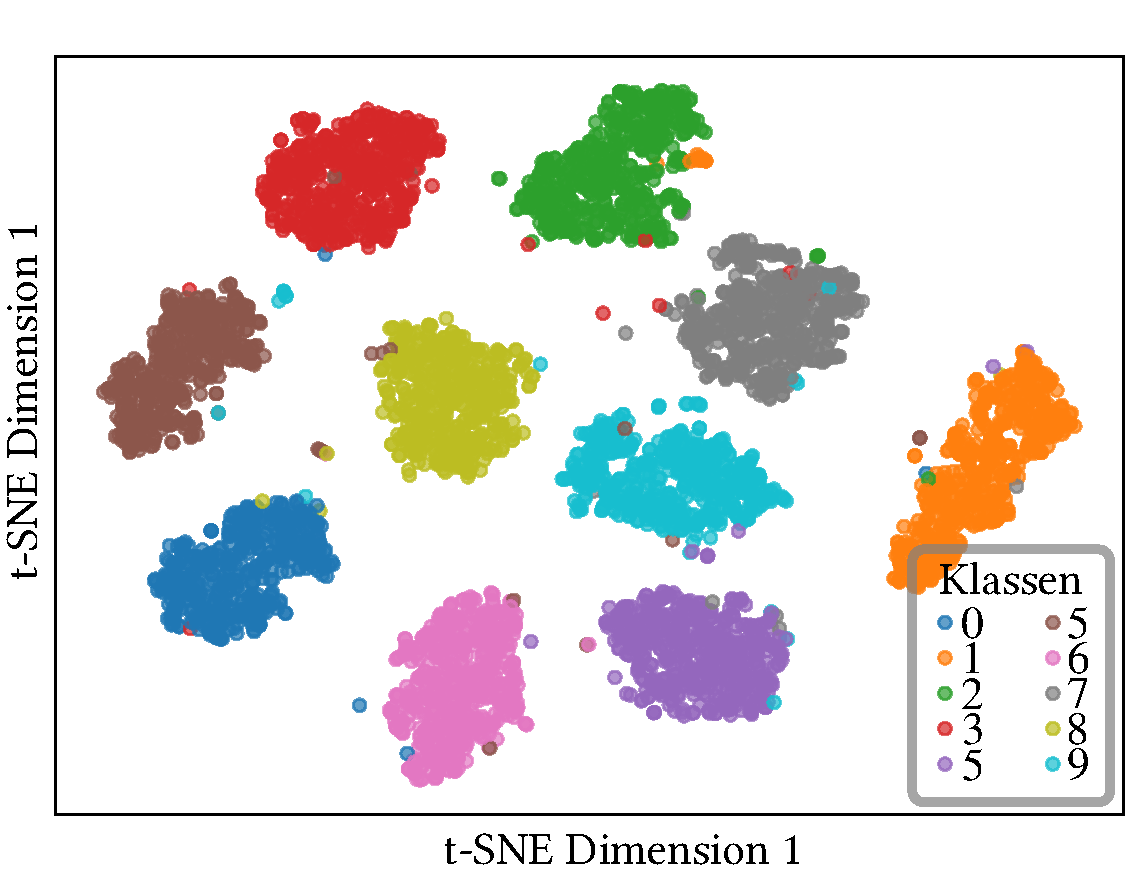
\includegraphics[width=\textwidth]{Figures/scatter_good.pdf}
    \end{subfigure}
    \caption{Zwei Scatterplots.
    Beide Scatterplots visualisieren den Merkmalsraum eines Klassifikators, links nach der ersten Epoche des Trainings, rechts nach 25 Epochen.
    Mithilfe der \ac{tsne} wird die hochdimensionale interne Repräsentation der Merkmale in eine zweidimensionale Ansicht projiziert.
    Einige Stichproben des MNIST-Datensatzes sind in dieser zweidimensionalen Ansicht platziert und ihre Klassen sind farblich markiert.}
    \label{fig:scatter_tsne_example}
\end{figure}
\noindent 
Dreidimensionale Daten stellen eine besondere Herausforderung für die Klassifikation dar \cite{Tran2018}.
Vortrainierte Methoden der 2D-Klassifikation wie \ac{cnn}-Encodern können auf einzelne Schichten eines 3D-Volumens angewandt werden, und die extrahierten Merkmale können anschließend aneinandergereiht werden, aber explizite 3D-Methoden sind oft besser \cite{Feichtenhofer2020}.
Die Methoden können auch an dreidimensionale Daten angepasst werden, indem ihre 2D-Operationen auf drei Dimensionen ausgeweitet werden, wodurch der Rechenaufwand steigt \cite{Carreira2017}.
Angepasste Methoden wie 3D-\acp{cnn} sind nicht in der Lage, Beziehungen zu erfassen, wenn die relevanten Bildregionen räumlich weit voneinander entfernt sind und schräg in den drei Dimensionen verteilt sind \cite{Tran2015}. 
Um dieses Problem zu lösen, schlägt die Literatur self-attention-Mechanismen über die Z-Dimension vor, die auch nicht-lokale Informationen erfassen \cite{Bertasius2021, Wang2018}. 
\section{Literaturrecherche}
\subsection{Benchmark}\label{sec:bench}
Da das Annotieren von Zelldaten für die Segmentierung mit erheblichem manuellen Aufwand verbunden ist und zusätzlich Expertenwissen voraussetzt, sind Datensätze hierfür selten.
Einige prominente Datensätze mit Annotationen für eine Instanzsegmentierung, deren Domänen zu den Zieldaten der Anwendung dieser Arbeit \textit{ähnlich} sind, sind:  
\begin{itemize}
    \item LiveCell \cite{edlund2021livecell}, ein manuell annotierter und von Expert*Innen validierter Datensatz aus 5.239 2D-Bildern. 
    Die Daten sind mit Phasenkontrastmikroskopie gesammelt und enthalten 1.686.352 individuelle Zellen von acht verschiedenen Zelltypen.
    \item YeaZ \cite{dietler2020YeaZ}, ein zweiteiliger Datensatz von Hefe-Zellen aus 87 Phasenkontrast-Bildern mit insgesamt 10.422 Zellen und 614 Hellfeld-Bildern mit insgesamt 3.841 Zellen in 6 Beleuchtungsstufen aufgenommen. Die Annotationen sind semi-manuell erstellt, da die Phasenkontrast-Bilder manuell und die Lichtfeld-Bilder aus den Phasenkonstrast-Segmentierungsmasken annotiert wurden. 
    \item DeepBas \cite{holden2021deepbacs, cspahn2021deepbacs}, ein Datensatz von \textit{B. subtilis strain SH130} Bakterien. Er besteht aus Weitfeldaufnahmen (Fluoreszenz), aufgenommen mit einem inversen Mikroskop, bestehend aus sieben manuell annotierten Bildern mit je 46 bis 335 Zellen.
    \item die Cell Tracking Challenge \cite{ulman2017cellTrackingChallenge}, eine Sammlung aus 13 Datensätzen verschiedener Mikroskopiemodalitäten, die sich zur Messung der Segmentierungs- und Verfolgungsfähigkeiten für verschiedene Zelltypen eignen.
    \item MoNuSeg \cite{kumar2017MoNuSeg}, eine Zusammenstellung manuell annotierter Gewebeschnitte aus sieben verschiedenen Organen. Über 21.000 Zellen sind pro Bild in den 30 Bildern mit verschiedenen Färbungen und Aufnahmetechniken verteilt.
    \item TissueNet \cite{greenwald2022Tissuenet} ist ein umfassender Datensatz mit über 1.000.000 Zellen aus verschiedenen Gewebearten und unterschiedlichen Aufnahmetechniken.
    \item S\_BIAD1518 \cite{Kromp2020_Dataset, chen20223_Dataset}, ein Datensatz, der neben manuell annotierten Bildern von acht verschiedenen Zellarten synthetisch erzeugte Daten enthält. Mithilfe von SpCycleGAN \cite{fu2018cycleGAN} wurden dazu auf Basis simulierter Annotationen Bilder generiert, die anstreben, die Merkmale der realen Bilder zu reproduzieren. Es handelt sich um 3D-Multispektraldaten, aufgenommen mittels Fluoreszenzbildgebung. 
\end{itemize}
Aufgrund des geringen Volumens an frei zugänglichen Daten sind diese Sammlungen auch für das Training von Segmentierungsnetzen begehrt. 
Neben annotierten Datensätzen bietet die Literatur auch Methoden zum eigenständigen Erzeugen domänenspezifischer Datensätze \cite{Abay2019, Raghunathan2021, Nikolenko2021, Choi2017, Lu2023}.
Beispielsweise können 3D-Trainingsdaten mit realistischer Zellform und -ausrichtung sowie umgebenden Markern synthetisch erzeugt und durch ein Generative Adversarial Network an eine gewünschte Bilddomäne angepasst werden \cite{bruch2025}. 

\subsection{Segmentierungsmodelle}
Foundation-Modelle sind für viele moderne \ac{ki}-Anwendungen unerlässlich \cite{bommasani2021foundationmodels}. 
Sie werden zunächst für allgemeine Aufgaben vortrainiert und anschließend auf spezifische Anwendungen angepasst (fine-tuning), meist unter Einfrieren von Teilen der Gewichte \cite{Yosinski2014}.
Auch Segmentierungsmodelle profitieren stark von umfangreichem Vortraining \cite{dippel2022segmentation}. 
In der aktuellen Forschung werden verschiedene Foundation-Modelle zur Segmentierung angewandt \cite{wang2021max,zou2023segment,jain2023oneformer,li2023mask}.
Ein prominentes Exemplar ist das \ac{sam} von Meta AI \cite{kirillov2023sam} (siehe Abb. \ref{fig:SAM_Architektur}). 
Es besteht aus einem Bild-Encoder, einem Prompt-Encoder und einem Masken-Decoder. 
\begin{figure}[H]
    \centering
    \includegraphics[width=1\linewidth]{Figures/SAM_Architecture.png}
    \caption{Architektur des \ac{sam}-Modells. 
    Eingabebilder werden durch einen Bildencoder in Repräsentationen umgewandelt. 
    Zusätzliche optionale Hinweise zum zu segmentierenden Objekt werden durch Bildfaltungen oder einen Prompt-Encoder repräsentiert. 
    Anschließend prädiziert der Decoder mehrere mögliche Masken und die zugehörigen Zuversichtlichkeiten \cite{kirillov2023sam}.}
    \label{fig:SAM_Architektur}
\end{figure}
\noindent
Als Bild-Encoder dient ein Vision Transformer \cite{dosovitskiy2020ViT} mit Vortraining als Masked Autoencoder \cite{he2022mae} und zusätzlichem Training für höhere Bildauflösung.
Der Prompt-Encoder ist mehrstufig.
Ein angelernter Positional Encoder generiert Repräsentationen aus Positions-Nutzereingaben wie Punkten und Boxen.
Für textuelle Prompts wird der Encoder des CLIP-Modells \cite{Radford2021} verwendet.
Außerdem werden Bildfaltungen als Encoder auf Maskeneingaben angewandt.
Mithilfe dieser Encoder wird dem Modell eine Repräsentation des zu segmentierenden Bildes sowie optional Hinweise auf das erwünschte Ergebnis bereitgestellt, die bereits semantische Informationen und abstrakte Bildmerkmale enthalten.
Aus diesen Repräsentationen generiert der Decoder anschließend mehrere mögliche Masken mit zugehörigen Zuversichtlichkeiten, aus denen ein finales Segmentierungsergebnis ausgewählt wird.\\ [0.5\baselineskip]
Das \ac{sam}-Modell wurde bereits für viele explizite Mikroskopie-Zelldaten-Anwendungen angepasst \cite{archit2025samfine, israel2023samfine, vandeloo2025samfine}. 
Auch für bestehende biologische Segmentierungsanwendungen, wie etwa Cellpose\cite{stringer2021cellpose}, wurde \ac{sam} auf Zelldaten angepasst \cite{pachitariu2025samcellpose}.
Dieser \textit{Fine-tune} nennt sich CellposeSAM.
Er kombiniert den Bild-Encoder von \ac{sam} mit dem \linebreak \textit{Flow}-Segmentierungsansatz von Cellpose.
Dabei generiert der Bild-Encoder direkt Vektoren, die Zwischenrepräsentationen, sogenannte \textit{Flows}, darstellen.
Diese \textit{Flows} werden pixelweise zu einem Gradientenfeld überführt.
Mithilfe der Gradienten werden Objektinstanzen vorhergesagt.
Abb. \ref{fig:CellposeSAM} zeigt diesen Ablauf als Diagramm.
\begin{figure}[H]
    \centering
    \includegraphics[width=0.98\linewidth]{Figures/CellposeSAM_Diagramm.png}
    \caption{Ablauf des CellposeSAM-Modells. 
    Eingabebilder werden durch einen Bild-Encoder (ViT-L) direkt zu sogenannten \textit{Flows} umgeformt, einer Repräsentation von vorhergesagten Objektmerkmalen, deren Werte von der relativen Position innerhalb des detektierten Objekts abhängen. 
    Die Gradienten der Flows werden verfolgt (gradient tracking) und aus dem daraus entstehenden Gradientenfeld werden Segmentierungsinstanzen (ROIs) vorhergesagt \cite{pachitariu2025samcellpose}.}
    \label{fig:CellposeSAM}
\end{figure}
\noindent
Deepcell \cite{van2016deepcell,bannon2021deepcell,greenwald2022deepcell} bietet weitere Zellsegmentierungsmodelle.
Das Deepcell-Caliban-Modell \cite{moen2019DeepcellCaliban} nutzt als Encoder eine EfficientNetV2L-Architektur \cite{Tan2021}, an deren Ausgabeschichten eine Pyramidenstruktur zur Merkmalsfusion angeschlossen ist. 
Eine Besonderheit des Netzes ist, dass Eingabebildern zusätzlich Koordinatenkarten hinzugefügt werden.
Als Decoder dienen drei Segmentierungsköpfe, die verschiedene Transformationen der annotierten Trainingsmasken vorhersagen.\\ [0.5\baselineskip]
In der Literatur ist außerdem das nnU-Net \cite{isensee2021nnu} sehr verbreitet, ein Segmentierungsframework, das sich automatisch an neue biomedizinische Aufgaben anpasst.
Es konfiguriert Vorverarbeitung, Netzwerkarchitektur, Training und Nachbearbeitung dynamisch auf Basis der Eigenschaften des jeweiligen Datensatzes. 
Die Leistungsfähigkeit des Ansatzes ergibt sich nicht aus einer neuen Architektur oder einer neuen Lernmethode, sondern aus der konsequenten Automatisierung und Systematisierung von Entwurfsentscheidungen.

\subsection{Klassifikator}
Für Klassifikatoren werden in der Regel nur Encoder vortrainiert.
Der Klassifikations-Kopf muss an die Klassen des vorliegenden Problems angepasst werden \cite{Plested2022, Yosinski2014, Dippel2022}.
State-of-the-Art für Bild-Encoder sind \acp{cnn} oder \acp{vit}, die auf dem ImageNet-Datensatz \cite{Russakovsky2015} vortrainiert werden \cite{You2018, Kornblith2019}.
Klassifikatoren profitieren stark von ImageNet-Vortraining \cite{Beyer2020, Recht2019}.\\[0.5\baselineskip]
\textbf{ResNet} ist ein Residual Neural Network, ein \ac{cnn} mit sogenannten residual connections \cite{He2016}.
Diese residual connections verbinden den Ein- und Ausgang modularer Faltungsschichten und verbessern die Leistungsfähigkeit tiefer neuronaler Netze \cite{He2016, He2015, srivastava2015highway} (siehe Abb. \ref{fig:ResDiagramms} a).
In ihrem Paper stellen die Autoren fünf unterschiedlich tiefe Varianten der \textbf{ResNet}-Architektur vor.
Jede Variante enthält fünf Blöcke mit residual connections.
Die Blöcke bestehen aus Faltungen mit verschiedenen Kernelgrößen und Strides, batch normalization \cite{Ioffe2017} und der ReLU \cite{Nair2010} Aktivierungsfunktion.\\[0.5\baselineskip]
\textbf{EfficientNet V2} ist ein Nachfolger der EfficientNet-Modellfamilie \cite{Tan2021, Tan2019}.
Die Architektur basiert auf modularen Blöcken von Bildfaltungsoperatoren mit besonders kleinen Faltungskernen und Squeeze-and-Excitations, genannt MBConv \cite{Tan2019, Sandler2018} und \linebreak Fused-MBConv \cite{Gupta2019} (siehe Abb. \ref{fig:ResDiagramms} b).\newline
\begin{figure}[H]
    \centering
    \includegraphics[width=0.98\textwidth]{Figures/Convs.pdf}
    \caption{Diagramme a) der Residual Connections \cite{He2016} und b) der MBConv-Blöcke und der Fused-MBConv-Blöcke \cite{Tan2021}.}
    \label{fig:ResDiagramms}
\end{figure}
\noindent
\textbf{ConvNeXt} \cite{Liu2022} ist eine \ac{cnn}-Modellfamilie mit besonders großen Faltungskernen. 
Die \textbf{ConvNeXt}-Architektur umfasst fünf modulare Blöcke mit Faltungen und residual connections, wie die ResNet-Architektur \cite{He2016}.
Allerdings verändert dabei \textbf{ConvNeXt} einige Details der ResNet-Architektur, wie beispielsweise die GeLU-Aktivierungsfunktion \cite{Hendrycks2016} und layer normalization \cite{Ba2016}.\\ [0.5\baselineskip]
Swin Transformer \cite{liu2021} ist eine beliebte Modellfamilie der \acp{vit}.
Ihr Nachfolger, die \textbf{Swin Transformer V2}-Familie \cite{Liu2022a}, vergrößert die Modelle weiter.
Die Architektur kombiniert Bildausschnitte mit einem Positionsbias.
Hierzu werden ein Bildfenster $z$ und dessen relative Koordinaten im Bild, $\Delta x$ und $\Delta y$, in einem attention-Mechanismus zusammengeführt.
Die Positionen werden in einem MLP-Netz verarbeitet, während das Bildfenster mit drei verschiedenen Gewichtsmatrizen multipliziert wird.
Mithilfe einer Kosinusähnlichkeitsfunktion, der Softmax-Funktion \cite{Bridle1989}, der elementweisen Multiplikation sowie der Addition werden diese Ergebnisse in einen Merkmalsraum überführt.
Zwei layer normalizations \cite{Ba2016}, ein weiteres MLP-Netz und residual connections vervollständigen anschließend den modularen \textbf{Swin Transformer V2}-Block.
Dieser Aufbau ist in Abb. \ref{fig:SwinArchitecture} im Anhang dargestellt. 
Der Abschnitt \ref{supp:swin} des Anhangs zeigt die Architektur als Diagramm.
\section{Offene Probleme}
Einzelne Myotuben lassen sich nicht mithilfe eines Segmentierungsmodells aus der Literatur instanzsegmentieren.
Selbst für Expert*Innen sind in dichten Strukturen Myotuben-Instanzen nicht immer eindeutig trennbar.
Nicht viele Segmentierungsmodelle für Nuclei sind erhältlich, insbesondere für dreidimensionale Daten.
Die verfügbaren Modelle verhalten sich je nach Datensatz unterschiedlich, und ihre Eignung für bestimmte Aufgaben muss in jeder Anwendung individuell geprüft werden.
Die Daten der vorliegenden Arbeit wurden gemäß dem Protokoll in Couturier et al. \cite{Couturier2024} erstellt und umfassen Myotubenkulturen sowie deren Nuclei und sind mit insgesamt fünf verschiedenen Fluoreszenzmarkern versehen.
Für diese spezifischen Aufnahmebedingungen und Marker der vorliegenden Daten gibt es keinen angepassten Klassifikator.
Der Erfolg eines Übertrags verschiedener vortrainierter Encoder und etablierter Methoden auf die vorliegenden Daten ist unvorhersehbar, da sich die gelernten Merkmalsräume möglicherweise nicht für die Klassifikation der neuartigen dreidimensionalen Daten eignen.
Eine weitere Fragestellung ist deshalb, wie Klassifikationsmethoden mit der Kombination der Marker umgehen. 
Für jeden Datensatz mit neuen Zellkernklassen und Aufnahmebedingungen muss nicht nur ein neues Modell trainiert, sondern auch Methoden- und Hyperparameteroptimierung durchgeführt werden, um optimale Klassifikatorleistung zu erzielen.
Des Weiteren ist der Umgang mit dreidimensionalen Daten, insbesondere in Umgebungen mit geringer Rechenleistung, ein offenes Problem.
Diverse Lösungen existieren, um dreidimensionale Daten mit Expertenwissen zu versehen.
Diesen Lösungen fehlt bislang ein Arbeitsablauf, der Daten unmittelbar segmentiert und vorbereitet, um relevante Bildausschnitte direkt aus dem Datensatz zu extrahieren, sodass Expert*Innen ausschließlich annotieren müssen.
\newpage
\section{Zielsetzung}
Im Zuge der vorliegenden Arbeit soll die automatische Extraktion interpretierbarer Eigenschaften der Myotubenkulturen ermöglicht werden.
Zu diesem Ziel definiert die vorliegende Arbeit folgende Zwischenziele:
\begin{itemize}
    \item Es soll ein Segmentierungsmodell gefunden werden, das die Eigenschaften wie Zellkernvolumina und die lokale Nucleidichte möglichst unverändert aus den vorliegenden, dreidimensionalen Daten extrahieren kann.
    Dazu wird ein neues Bewertungskriterium für die Instanzsegmentierung eingeführt und auf einige etablierte Modelle angewandt.
    \item Das Segmentierungsmodell soll dann genutzt werden, um einen Ablauf zu schaffen, in dem Expert*Innen die Klassen der Nuclei besonders zeiteffizient annotieren können, um einen Klassifikator zu trainieren.
    Durch das Anreichern dreidimensionaler Daten mit den Segmentierungsmasken und das automatische Fokussieren einzelner Nuclei sollen sowohl die Rechenzeit optimiert werden als auch der Aufwand, einzelne Nuclei entlang drei Dimensionen zu suchen, eliminiert werden.
    Hierzu wird eine neue Anwendung entwickelt, die 3D-Zelldaten liest und anschließend eine Oberfläche zur Annotierung bereitstellt.
    \item Die entstehenden Annotationen sollen direkt in einen Trainingsablauf für Klassifikatoren integriert werden.
    Hierbei müssen Klassifikatoren mit dreidimensionalen Daten variabler Tiefe umgehen können.
    Ein ausführlicher Methodenvergleich verschiedener Encoder, Klassifikations-Köpfe, Vorverarbeitungsmethoden sowie Vortrainingsmethoden soll für Nutzer*Innen ohne Programmierkenntnisse ermöglicht werden.
    Dazu wird eine neue Anwendung entwickelt, die die erstellten Annotationen und Segmentierungsmasken nutzt, um einen Klassifikator zu trainieren.
    Nutzer*Innen können in einer grafischen Oberfläche verschiedene Methoden zum Vergleich auswählen, und in einem automatisierten Prozess werden Klassifikatoren aller Kombinationen trainiert und verglichen.
    \item Außerdem sollen die ausgelesenen Eigenschaften der eingegebenen Zelldaten leicht zugänglich sein.
    In einer weiteren neuen Anwendung werden automatisch die Vorhersagen des Klassifikators mit dem besten Ergebnis im Methodenvergleich genutzt, um Nutzer*Innen Graphen mit den Eigenschaften der Zellkultur darzubieten.
    \item Zuletzt sollen alle neu entwickelten Module zu einer Gesamtanwendung zusammengefasst und getestet werden.
    In einer Parameterbestimmung wird das Optimum für die vorliegenden Aufnahmen explizit mithilfe der neuen Anwendung bestimmt.
\end{itemize}